%%%%%%%%%%%%%%%%%%%%%%%%%%%%%%%%%%%%%%%%%%%%%%%%%%%%%%%%%%%%%%%%%%%%%%%%%%%%%%%%%%%%%%%%%%%	
% source1 : http://sdz.tdct.org/sdz/creez-vos-diaporamas-en-latex-avec-beamer.html
% source2 : https://deic.uab.cat/~iblanes/beamer_gallery/index_by_theme_and_color.html
% logo https://latex-beamer.com/tutorials/logo-beamer/
%%%%%%%%%%%%%%%%%%%%%%%%%%%%%%%%%%%%%%%%%%%%%%%%%%%%%%%%%%%%%%%%%%%%%%%%%%%%%%%%%%%%%%%%%%%	
\documentclass{beamer}
%%%%%%%%%%%%%%%%%%%%%%%%%%%%%%%%%%%%%%%%%%%%
\usepackage[frenchb]{babel}
\usepackage[T1]{fontenc}

%%%%%%%%%%%%%%%%%%%%%%%%%%%%%%%%%%%%%%%%%%%%
\setbeamertemplate{navigation symbols}{} % Supprimer la navigation
\usetheme{CambridgeUS} %Theme
\usecolortheme{dolphin} 
\usefonttheme{default}

%%%%%%%%%%%%%%%%%%%%%%%%%%%%%%%%%%%%%%%%%%%%
% definir la couleur du titre http://sdz.tdct.org/sdz/creez-vos-diaporamas-en-latex-avec-beamer.html#Modesdecouleurs
\definecolor{myblue1}{RGB}{188,188,228} 

%%%%%%%%%%%%%%%%%%%%%%%%%%%%%%%%%%%%%%%%%%%%
%https://tex.stackexchange.com/questions/151306/beamer-titlepage-picture
\addtobeamertemplate{title page}{
\includegraphics[scale=.05]{logoUmons.png} \hfill 
\includegraphics[scale=0.19]{index.png} \\[.2cm]}{}
\setbeamercolor{title}{bg=myblue1,fg=black}

%%%%%%%%%%%%%%%%%%%%%%%%%%%%%%%%%%%%%%%%%%%%
% set captions of figure with numbers, 
% source : https://latex-beamer.com/tutorials/beamer-figure/
\setbeamertemplate{caption}[numbered]

%%%%%%%%%%%%%%%%%%%%%%%%%%%%%%%%%%%%%%%%%%%%
% Definir la couleur des blocks, 
% source:  https://perso.crans.org/besson/internship-mva-2016/slides/naereenbeamer.sty
\setbeamercolor{block body}{bg=normal text.bg!90!black}
\setbeamercolor{block title}{use={normal text,example text},bg=myblue1}

%%%%%%%%%%%%%%%%%%%%%%%%%%%%%%%%%%%%%%%%%%%%
% Note en bas de page
%Source : https://www.xm1math.net/doculatex/notesbasdepage.html
\AddThinSpaceBeforeFootnotes % à insérer si on utilise \usepackage[french]{babel}
\FrenchFootnotes % à insérer si on utilise \usepackage[french]{babel}

%%%%%%%%%%%%%%%%%%%%%%%%%%%%%%%%%%%%%%%%%%%%
% How to change the color of \href links... for real https://tex.stackexchange.com/questions/13423/how-to-change-the-color-of-href-links-for-real
\definecolor{links}{HTML}{2A1B81}
\hypersetup{colorlinks,linkcolor=,urlcolor=links}

%%%%%%%%%%%%%%%%%%%%%%%%%%%%%%%%%%%%%%%%%%%%%%%%%%%%%%%%%%%%%%%%%%%%%%%%%%%%%%%%%%%%%%%%%%%	

\title[Lecture et rédaction scientifique]{Lecture et rédaction scientifique \\ Skip list}
\author[Skip List (Y. KAZZOUL)]{ 
	Présenté par Youness KAZZOUL \\[0.8cm] 
	Directeur : Gwenaël JORET \\[0.1cm] 
	Université de Mons - Faculté des Sciences}
\date[Umons - 2022]{\\[-2cm]\today}

%%%%%%%%%%%%%%%%%%%%%%%%%%%%%%%%%%%%%%%%%%%%%%%%%%%%%%%%%%%%%%%%%%%%%%%%%%%%%%%%%%%%%%%%%%%	

\begin{document}	
	\maketitle	
	
%%%%%%%%%%%%%%%%%%%%%%%%%%%%%%%%%%%%%%%%%%%%%%%%%%%%%%%%%%%%%%%%%%%%%%%%%%%%%%%%%%%%%%%%%%%	

	\begin{frame}{Table des matières}
	\setbeamertemplate{section in toc}[sections numbered]
	\tableofcontents%[hideallsubsections]
	~\end{frame}

%%%%%%%%%%%%%%%%%%%%%%%%%%%%%%%%%%%%%%%%%%%%%%%%%%%%%%%%%%%%%%%%%%%%%%%%%%%%%%%%%%%%%%%%%%%	
	
\section[Introduction]{Introduction}
\begin{frame}
	\frametitle{Introduction}
	
	\textbf{William Worthington Bill Pugh Jr} \\
	\begin{columns}		
		\column{0.2\textwidth}		
		\begin{figure}
			\centering	
			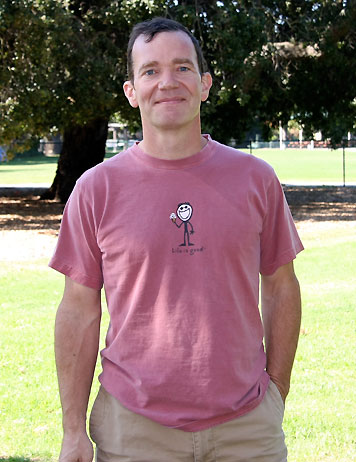
\includegraphics[width=1\textwidth]{bill.jpg}	\\			
		\end{figure}
		
		\column{0.1\textwidth}
		
	\column{0.6\textwidth}	
	
	\begin{block}{Caractéristiques des skip lists \cite{ArticlePugh}} 
		\begin{itemize}
			\item Alternatives aux ABR équilibrés.	\\[.6cm]
			\item Algorithmes simples et rapides.  \\[.6cm]
			\item Équilibrage probabiliste et non forcée.

		\end{itemize}
	\end{block}	
	\end{columns}
	%\centering
	%~\\[.6cm]
	\begin{flushleft}
		{Source : \href{www.cs.umd.edu/~pugh/bio.html}{www.cs.umd.edu/~pugh/bio.html} 	}
	\end{flushleft}	
	
\end{frame}

%%%%%%%%%%%%%%%%%%%%%%%%%%%%%%%%%%%%%%%%%%%%%%%%%%%%%%%%%%%%%%%%%%%%%%%%%%%%%%%%%%%%%%%%%%%	

\section[Description]{Description}
\begin{frame}
	\frametitle{Description de skip list}
	
		\begin{figure}
			\centering			
			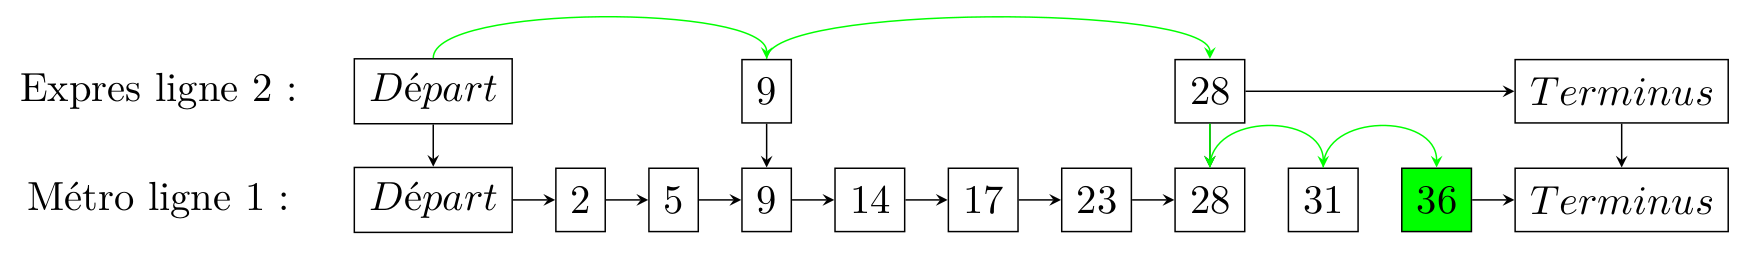
\includegraphics[width=1\textwidth]{discription.png}
			\caption{Analogie des Skip list avec le transport ferroviaire.}		
		\end{figure}	
	
	\centering
	{\footnotesize {Source: le code source développé figure en annexe.}}			

\end{frame}	

%%%%%%%%%%%%%%%%%%%%%%%%%%%%%%%%%%%%%%%%%%%%%%%%%%%%%%%%%%%%%%%%%%%%%%%%%%%%%%%%%%%%%%%%%%%	

\section[Algorithmes]{Algorithmes}
\subsection{Algorithme de Recherche}
{	
	\begin{frame}
			\frametitle{Algorithme de Recherche}				
				\begin{figure}
					\centering			
					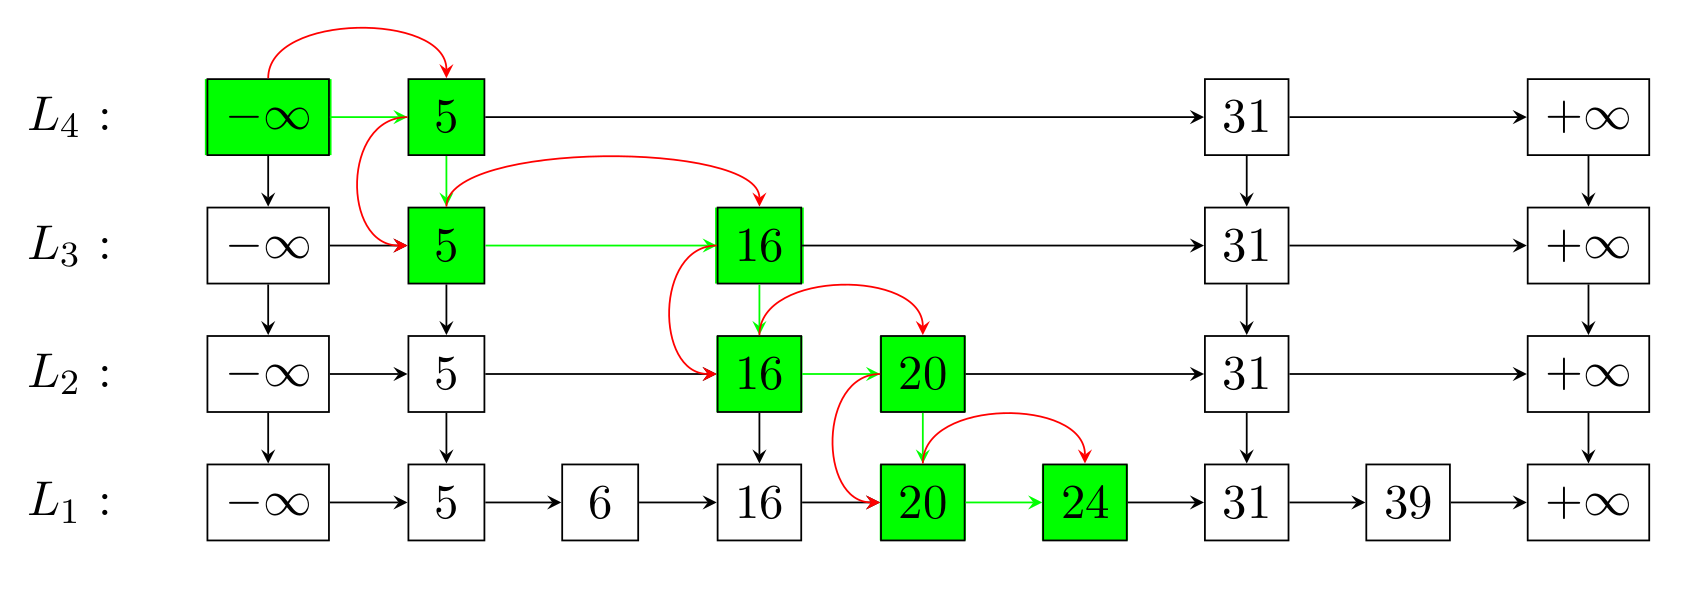
\includegraphics[width=0.9\textwidth]{recherche.png}
					\caption{Exemple de recherche de clé 24.}
				\end{figure}
			
			\centering
			{\footnotesize {Source: le code source développé figure en annexe.}}

	\end{frame}
}
%%%%%%%%%%%%%%%%%%%%%%%%%%%%%%%%%%%%%%%%%

\subsection{Algorithme de Randomisation}
{
\begin{frame}	
	\frametitle{Algorithme de Randomisation}
	
	\begin{block}{Objectifs d'algorithme de Randomisation \cite{ArticleHamel}} 
		~\\[.4cm]
	\begin{itemize}		
		\item Déterminer le niveau du noeud à insérer.\\[.4cm]
		\item Un algorithme de génération aléatoire (\textit{e.g.}, Pile ou Face).\\[.4cm]
		\item Temps d’exécution : 
		\begin{itemize} 
			\item Dépend de la séquence (ou de la séquence de piles-faces).\\[.4cm]
			\item Pire cas, avec une faible probabilité (\textit{e.g.}, seulement des piles).
		\end{itemize}
	\end{itemize}
		~\\[.4cm]
	\end{block}				
		
\end{frame}	
}

%%%%%%%%%%%%%%%%%%%%%%%%%%%%%%%%%%%%%%%%%
% Figures in Beamer – A detailed tutorial
% https://latex-beamer.com/tutorials/beamer-figure/

\subsection{Algorithme de Insertion}
{
	\begin{frame}	
%		\frametitle{Algorithme d'insertion} 
		~\\[-0.8cm]
		\begin{figure}
			\centering
			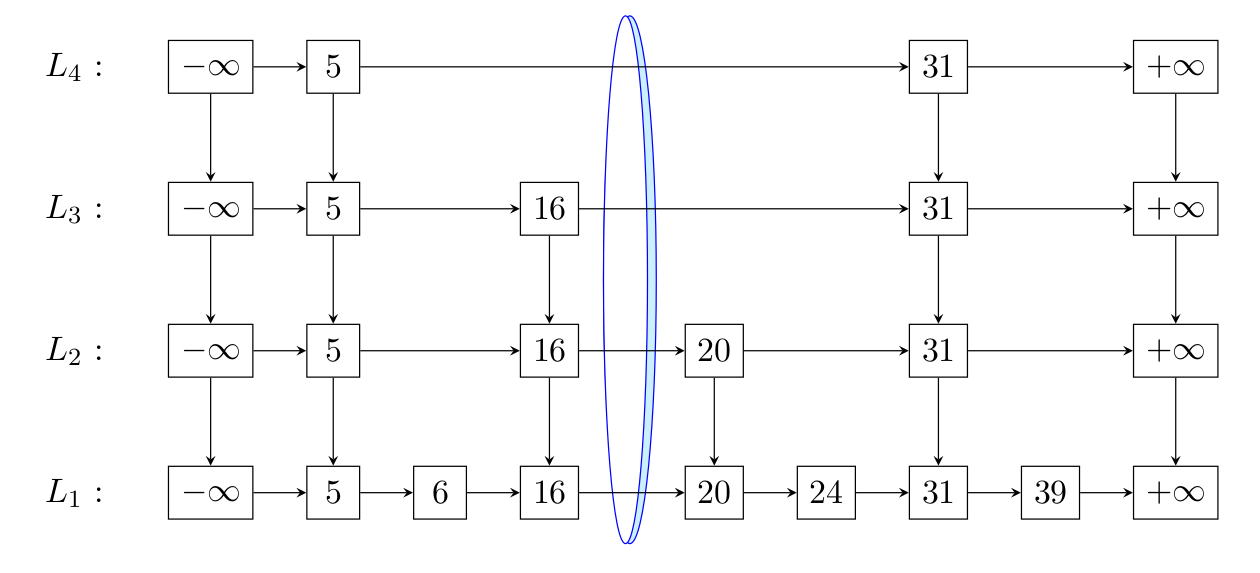
\includegraphics[height=0.35\textheight]{insert1.png}\\[-.4cm]
			\caption{Positionnement où la clé 18 va être insérée.} 
			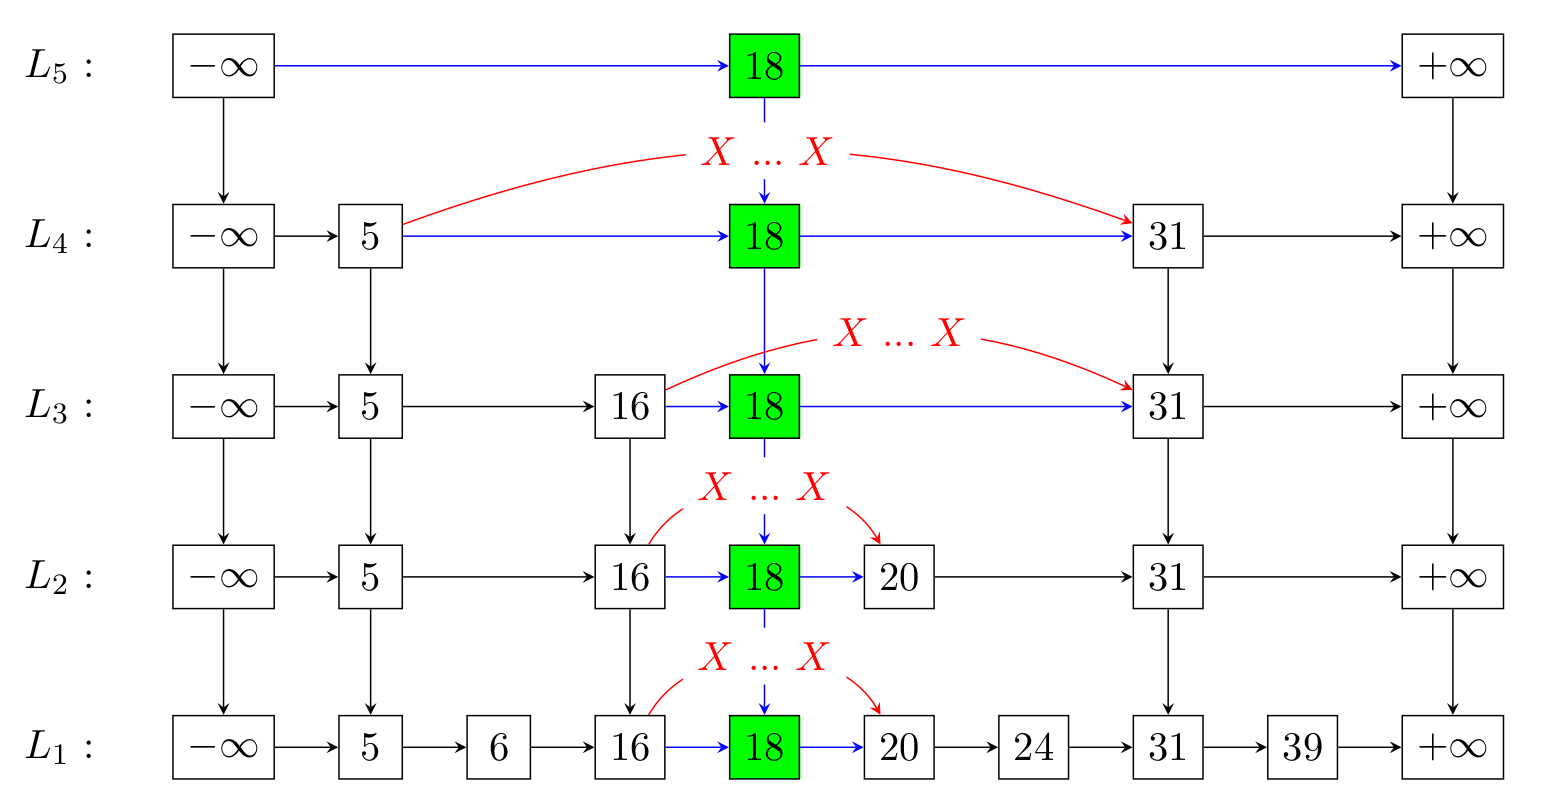
\includegraphics[height=0.38\textheight]{insert2.png}\\[-.4cm]
			\caption{Insertion de la clé 18, et mise à jours des pointeurs.}
		\end{figure}
	\centering
	{\footnotesize {Source: le code source développé figure en annexe.}}

	\end{frame}
}

%%%%%%%%%%%%%%%%%%%%%%%%%%%%%%%%%%%%%%%%%

\subsection{Algorithme de Suppression}
{
	\begin{frame}
%		Algorithme de Suppression
		~\\[-0.8cm]
		\begin{figure}
			\centering
			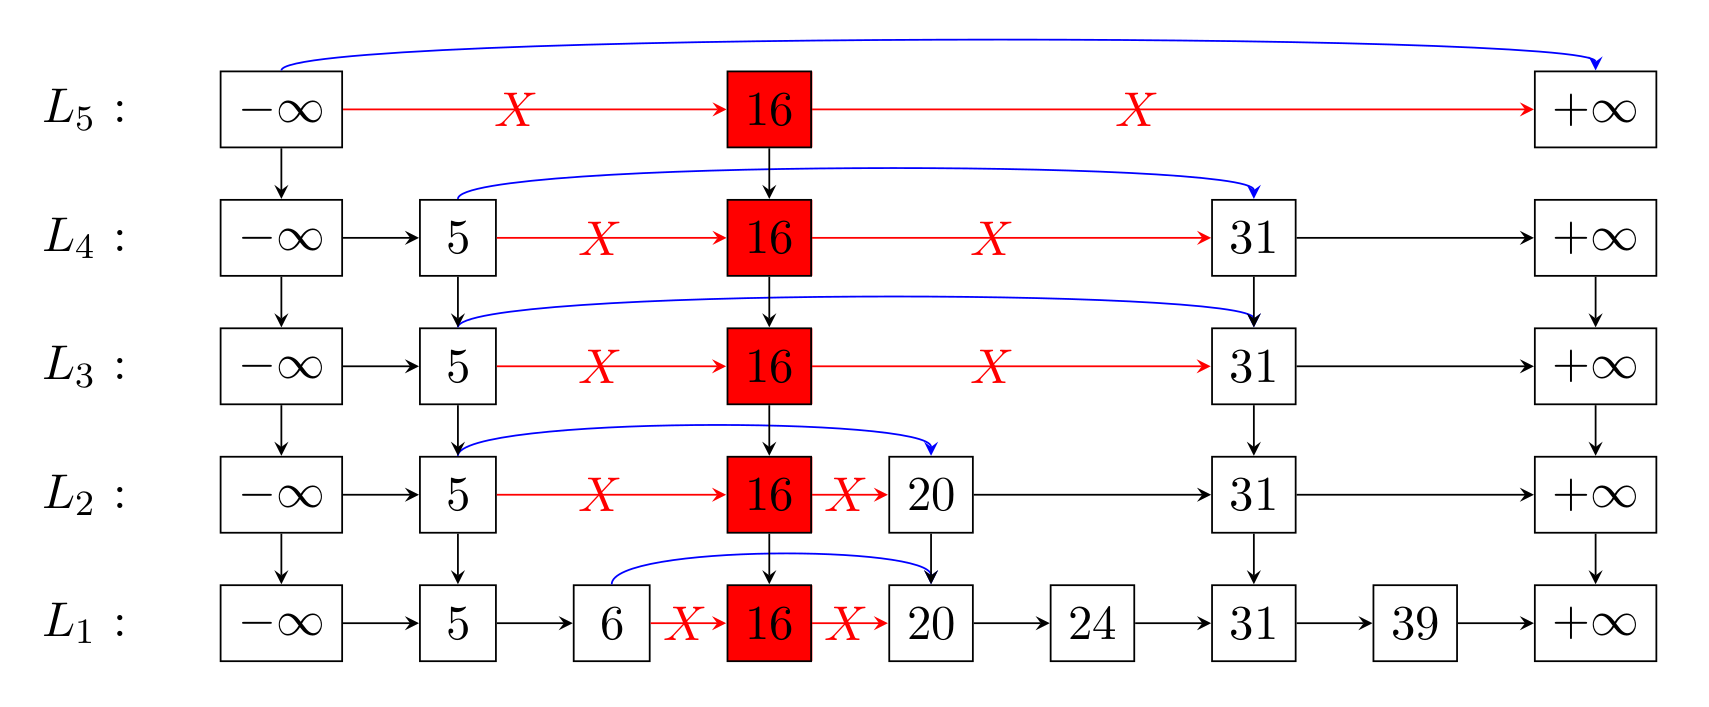
\includegraphics[height=0.38\textheight]{del1.png}\\[-.4cm]
			\caption{Localisation de la clé 16 avant la suppression.} 
			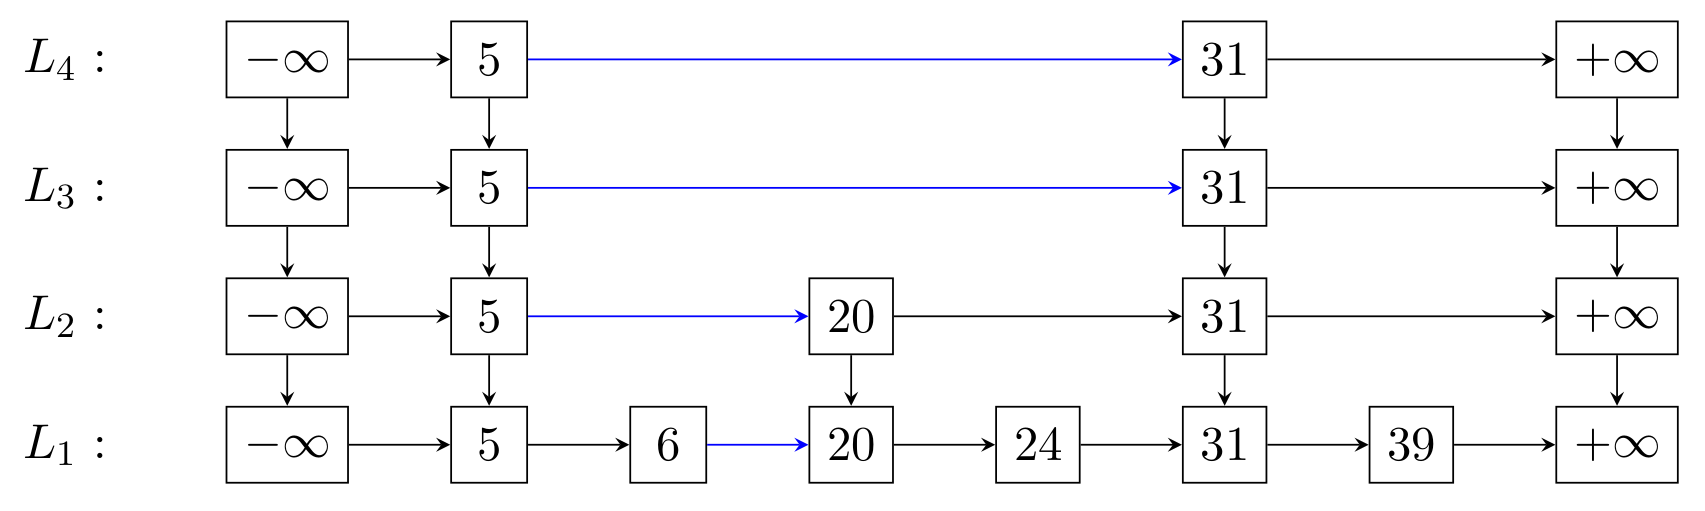
\includegraphics[height=0.3\textheight]{del2.png}\\[-.4cm]
			\caption{Suppression de la clé 16, et mise à jours des pointeurs.}			
		\end{figure}
	\centering
	{\footnotesize {Source: le code source développé figure en annexe.}}
	
	\end{frame}
}

%%%%%%%%%%%%%%%%%%%%%%%%%%%%%%%%%%%%%%%%%%%%%%%%%%%%%%%%%%%%%%%%%%%%%%%%%%%%%%%%%%%%%%%%%%%	

\section[Complexité]{Complexité}

\begin{frame}
	\frametitle{Complexité}
	
	Complexité temporelle :
		\begin{table}[h]  
		\centering
		\begin{tabular}{|c|c|c|}
			\hline
			Complexité  		&  Attendue        &  Pire          \\
			\hline
			Recherche   		& $\mathcal{O}(\log(n))$ &  $\mathcal{O}$(n)   \\	
			\hline
			Insertion   		& $\mathcal{O}(\log(n))$ &  $\mathcal{O}$(n)   \\	
			\hline
			Suppression 		& $\mathcal{O}(\log(n))$ &  $\mathcal{O}$(n)   \\	
			\hline
		\end{tabular}
		\caption{Complexité temporelle des Skip list.} 		
	\end{table}
	 
	 	~\\[.4cm]
	 	
	 Complexité spatiale est en $\mathcal{O}(n)$.
	 	 
\end{frame}	

%%%%%%%%%%%%%%%%%%%%%%%%%%%%%%%%%%%%%%%%%%%%%%%%%%%%%%%%%%%%%%%%%%%%%%%%%%%%%%%%%%%%%%%%%%%	

\section[Applications]{Applications} 

\begin{frame} 
	
	\frametitle{Applications}
	
	Les skip lists ont fait leur apparition dans plusieurs applications comme :
	~\\[.4cm]
	\begin{block}{Applications \cite{Wikipedia}}
		~\\[.4cm]
		\begin{itemize} %
		\item Redis «Remote Dictionary Server».\\[.4cm]	
		\item Bases de données \textit{e.g,} SingleStore. \\[.4cm]
		\item Serveurs Cyrus IMAP.	\\[.4cm]	
		\item Apache Portable Run-time.
		\item ...	
		\end{itemize}
	~\\[.4cm]
	\end{block}

\end{frame}	

%%%%%%%%%%%%%%%%%%%%%%%%%%%%%%%%%%%%%%%%%%%%%%%%%%%%%%%%%%%%%%%%%%%%%%%%%%%%%%%%%%%%%%%%%%%	

\section[Conclusion]{Conclusion}

\begin{frame}
	\frametitle{Conclusion}
	\begin{itemize}
		\item Le pire des cas diminue quand le nombre de nœuds augmente. \\[.2cm]
		\item Facile à mettre en œuvre. \\[.2cm]
		\item Un temps d'exécution en $\mathcal{O}(\log(n))$ dans le meilleur des cas pour toutes les opérations.\\[.2cm]
		\item Alternative aux arbres équilibrés. \\[.2cm]		
		\item Plus grande quantité de mémoire.

	\end{itemize}
	
\end{frame}	

%%%%%%%%%%%%%%%%%%%%%%%%%%%%%%%%%%%%%%%%%%%%%%%%%%%%%%%%%%%%%%%%%%%%%%%%%%%%%%%%%%%%%%%%%%%	

\begin{frame}  
	\frametitle{Annexe}
	
	Toutes les sources et l’intégralité de ce codes qu'ont servi à la rédaction de cette présentation se trouvent sur le document latex sur ce lien : \\[.5cm]
	\href{https://github.com/YounessKazzoul/Skip-lists}{https://github.com/YounessKazzoul/Skip-lists} 
	
\end{frame}

%%%%%%%%%%%%%%%%%%%%%%%%%%%%%%%%%%%%%%%%%%%%%%%%%%%%%%%%%%%%%%%%%%%%%%%%%%%%%%%%%%%%%%%%%%%	

\begin{frame}  
	\frametitle{References}
	\bibliographystyle{apalike}
	\bibliography{reference.bib} 	
\end{frame}

%%%%%%%%%%%%%%%%%%%%%%%%%%%%%%%%%%%%%%%%%%%%%%%%%%%%%%%%%%%%%%%%%%%%%%%%%%%%%%%%%%%%%%%%%%%	

\begin{frame}
	\frametitle{Questions}
	\begin{center}
		Questions 
	\end{center}
\end{frame}	






\end{document}
